% 图 1.2 —— 手工重建（两个三圆 Venn 面板）
%
% 做法同 1.1 / 2.1：看图定「是什么」，算法只在圈定区域内量「是多少」。
%
%   左面板  阴影 = A ∪ (B∩C)        右面板  阴影 = (A∪B) ∩ C
%   六个圆   实测 r = 92.1~92.7（取 92.6）；圆心见下
%            左面板少检了一个圆（B），按**右面板的同款偏移**补：
%            B−A = (88.7,−67.1)、C−A = (88.6,57.1) —— 书里两面板是同一套模板
%   阴影     45°，间距 8.6，线宽 3.0（族实测）
%   圆周     4.4pt（与 1.1 一致）
%   标签     A/B/C 的位置取实测框中心并补墨迹偏移；∪/∩ 按几何画（见 cupcap.py）；
%            括号左右由形状判正（glyphfix.py）—— 识别器原本把 `)` 认成了 `(`
\documentclass[12pt]{standalone}
\usepackage{fontspec}
\setsansfont{Arial}
\newfontfamily\mfallback{DejaVu Sans}
\usepackage{tikz}
\usetikzlibrary{patterns}

% 阴影线：45°，垂直间距 8.6 → 平铺边长 8.6*sqrt(2)=12.163
\pgfdeclarepatternformonly{hatch45b}
  {\pgfqpoint{-12.163pt}{-12.163pt}}
  {\pgfqpoint{12.163pt}{12.163pt}}
  {\pgfqpoint{12.163pt}{12.163pt}}
  {\pgfsetlinewidth{3.0pt}\pgfsetstrokecolor{black}%
   \pgfpathmoveto{\pgfqpoint{0pt}{0pt}}%
   \pgfpathlineto{\pgfqpoint{12.163pt}{12.163pt}}%
   \pgfusepath{stroke}}

\def\rC{92.6}
\def\wCirc{4.4}

\begin{document}
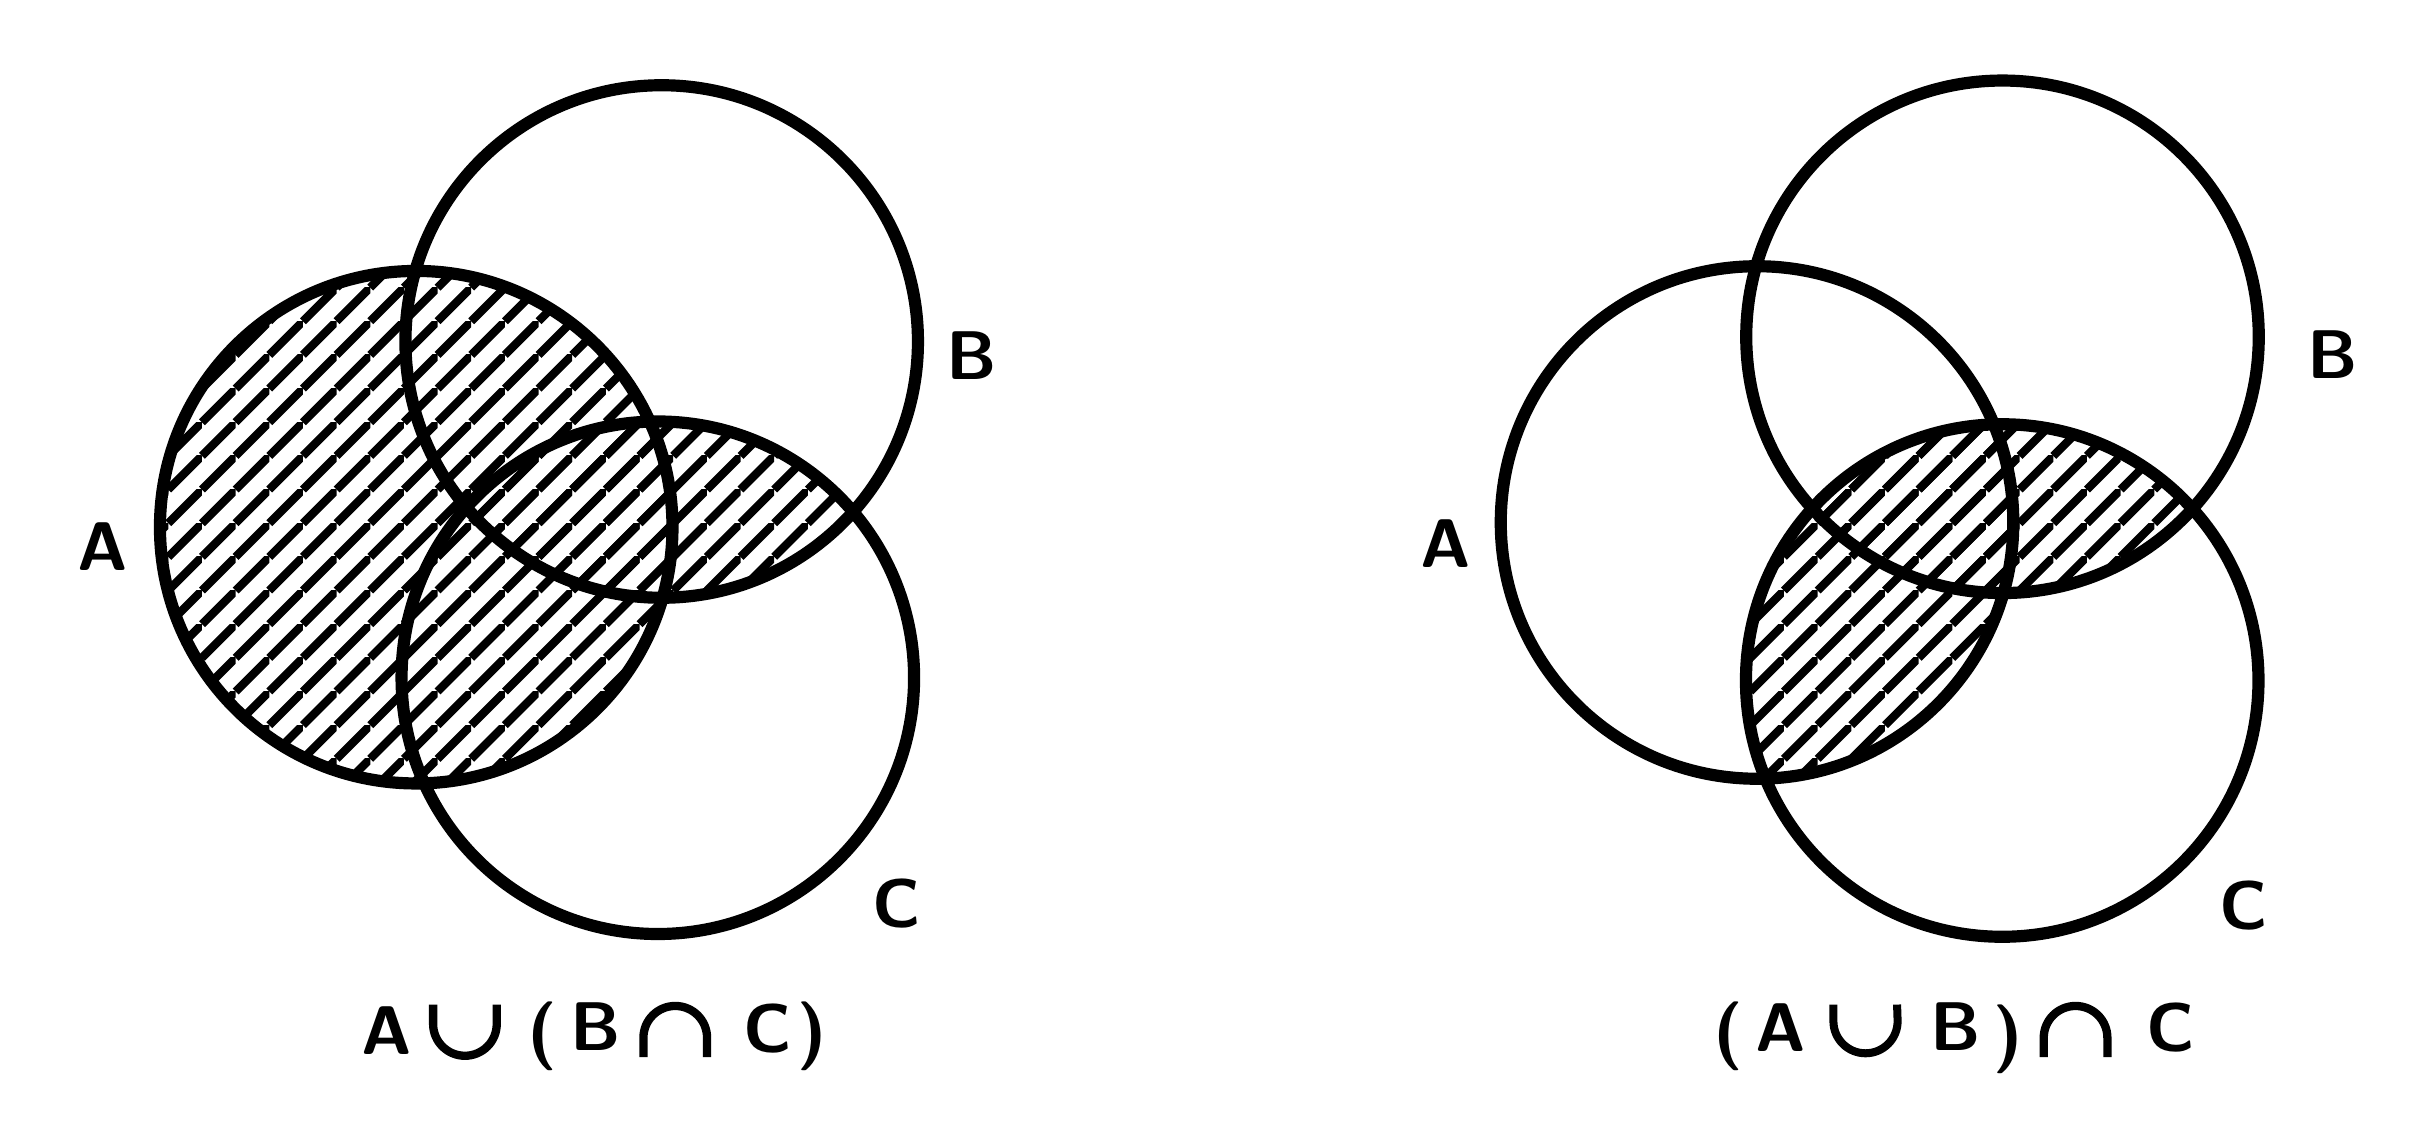
\begin{tikzpicture}[x=1pt, y=-1pt]
  % ── 圆心（实测；左面板 B 按右面板偏移补）──
  \coordinate (A1) at (140.4,180.5); \coordinate (B1) at (229.1,113.4); \coordinate (C1) at (227.7,234.9);
  \coordinate (A2) at (624.9,178.8); \coordinate (B2) at (713.6,111.7); \coordinate (C2) at (713.5,235.9);

  % ════ 左面板：A ∪ (B∩C) ════
  \begin{scope}                      % ① A 整圆
    \clip (A1) circle (\rC);
    \fill[pattern=hatch45b] (A1) circle (\rC);
  \end{scope}
  \begin{scope}                      % ② B∩C：夹到 B，再夹到 C
    \clip (B1) circle (\rC);
    \begin{scope}\clip (C1) circle (\rC);
      \fill[pattern=hatch45b] (B1) circle (\rC);
    \end{scope}
  \end{scope}
  \draw[line width=\wCirc] (A1) circle (\rC);
  \draw[line width=\wCirc] (B1) circle (\rC);
  \draw[line width=\wCirc] (C1) circle (\rC);

  % ════ 右面板：(A∪B) ∩ C ════
  \begin{scope}                      % 夹到 C，再填 A 与 B
    \clip (C2) circle (\rC);
    \fill[pattern=hatch45b] (A2) circle (\rC);
    \fill[pattern=hatch45b] (B2) circle (\rC);
  \end{scope}
  \draw[line width=\wCirc] (A2) circle (\rC);
  \draw[line width=\wCirc] (B2) circle (\rC);
  \draw[line width=\wCirc] (C2) circle (\rC);

  % ════ 面板内标签（实测框中心 + 墨迹偏移）════
  \node[anchor=center,inner sep=1.5pt,fill=white,font=\fontsize{27.2}{34.0}\selectfont] at (27.2,187.5) {\textsf{\textbf{\textit{A}}}};
  \node[anchor=center,inner sep=1.5pt,fill=white,font=\fontsize{29.6}{37.0}\selectfont] at (341.2,118.5) {\textsf{\textbf{\textit{B}}}};
  % 左面板的 C 识别器漏了，位置按右面板的同款偏移补（C−A 平移）
  \node[anchor=center,inner sep=1.5pt,fill=white,font=\fontsize{33.0}{41.3}\selectfont] at (314.0,316.5) {\textsf{\textbf{\textit{C}}}};
  \node[anchor=center,inner sep=1.5pt,fill=white,font=\fontsize{28.8}{36.0}\selectfont] at (512.6,186.5) {\textsf{\textbf{\textit{A}}}};
  \node[anchor=center,inner sep=1.5pt,fill=white,font=\fontsize{31.0}{38.8}\selectfont] at (832.8,118.0) {\textsf{\textbf{\textit{B}}}};
  \node[anchor=center,inner sep=1.5pt,fill=white,font=\fontsize{33.7}{42.1}\selectfont] at (800.8,317.3) {\textsf{\textbf{\textit{C}}}};

  % ════ 底部说明文字 ════
  % 左：A ∪ (B ∩ C)
  \node[anchor=center,inner sep=1.5pt,fill=white,font=\fontsize{28.8}{36.0}\selectfont] at (129.6,362.5) {\textsf{\textbf{\textit{A}}}};
  \draw[line width=3.0pt] (146.5,353.0) -- (146.5,360.0) arc (180:0:11.5) -- (169.5,353.0);
  \node[anchor=center,inner sep=1.5pt,fill=white,font=\fontsize{32.6}{40.7}\selectfont] at (186.0,364.5) {\textsf{\textbf{(}}};
  \node[anchor=center,inner sep=1.5pt,fill=white,font=\fontsize{30.2}{37.8}\selectfont] at (205.3,361.0) {\textsf{\textbf{\textit{B}}}};
  \draw[line width=3.0pt] (222.5,372.0) -- (222.5,365.0) arc (180:360:11.5) -- (245.5,372.0);
  \node[anchor=center,inner sep=1.5pt,fill=white,font=\fontsize{29.6}{37.0}\selectfont] at (267.3,361.8) {\textsf{\textbf{\textit{C}}}};
  \node[anchor=center,inner sep=1.5pt,fill=white,font=\fontsize{30.7}{38.4}\selectfont] at (283.5,364.5) {\textsf{\textbf{)}}};

  % 右：(A ∪ B) ∩ C
  \node[anchor=center,inner sep=1.5pt,fill=white,font=\fontsize{30.7}{38.4}\selectfont] at (614.5,364.5) {\textsf{\textbf{(}}};
  \node[anchor=center,inner sep=1.5pt,fill=white,font=\fontsize{28.8}{36.0}\selectfont] at (633.6,361.5) {\textsf{\textbf{\textit{A}}}};
  \draw[line width=2.9pt] (652.5,353.0) -- (652.5,359.0) arc (180:0:11.6) -- (675.5,353.0);
  \node[anchor=center,inner sep=1.5pt,fill=white,font=\fontsize{31.0}{38.8}\selectfont] at (696.8,361.0) {\textsf{\textbf{\textit{B}}}};
  \node[anchor=center,inner sep=1.5pt,fill=white,font=\fontsize{30.7}{38.4}\selectfont] at (715.5,365.5) {\textsf{\textbf{)}}};
  \draw[line width=3.0pt] (728.5,372.0) -- (728.5,365.0) arc (180:360:11.5) -- (751.5,372.0);
  \node[anchor=center,inner sep=1.5pt,fill=white,font=\fontsize{32.9}{41.2}\selectfont] at (774.3,361.3) {\textsf{\textbf{\textit{C}}}};

  \path[use as bounding box] (0,0) rectangle (852,388);
\end{tikzpicture}
\end{document}
